\documentclass[border=2pt]{standalone}
\usepackage{pgfplots}
\pgfplotsset{compat=1.18}
\usepackage{xcolor}

\definecolor{hdcblue}{RGB}{31,119,180}
\definecolor{matrixred}{RGB}{214,39,40}

\begin{document}
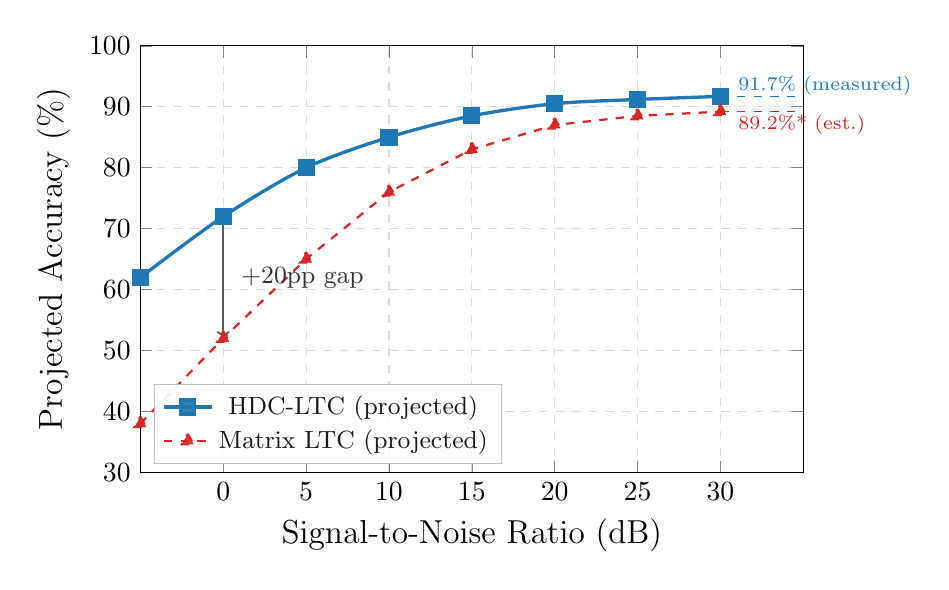
\begin{tikzpicture}
\begin{axis}[
    width=10cm,
    height=7cm,
    xlabel={Signal-to-Noise Ratio (dB)},
    ylabel={Projected Accuracy (\%)},
    xlabel style={font=\large},
    ylabel style={font=\large},
    xmin=-5, xmax=35,
    ymin=30, ymax=100,
    ytick={30,40,50,60,70,80,90,100},
    xtick={0,5,10,15,20,25,30},
    grid=both,
    grid style={dashed, gray!30},
    legend style={at={(0.02,0.02)}, anchor=south west, font=\small, draw=gray!50, fill=white, fill opacity=0.9},
    clip=false,
]

% HDC-LTC: graceful degradation (projected from HD theory)
% Based on distributed encoding: corrupting k/D dims loses k/D information
% At clean (30dB): 91.7%. Degrades slowly.
\addplot[hdcblue, very thick, smooth, mark=square*, mark size=2.5pt, mark options={fill=hdcblue}] coordinates {
    (-5, 62)
    (0, 72)
    (5, 80)
    (10, 85)
    (15, 88.5)
    (20, 90.5)
    (25, 91.2)
    (30, 91.7)
};

% Standard LTC: sharper degradation (projected)
% Matrix operations: corrupting entries alters learned mapping
\addplot[matrixred, thick, dashed, mark=triangle*, mark size=2.5pt, mark options={fill=matrixred}] coordinates {
    (-5, 38)
    (0, 52)
    (5, 65)
    (10, 76)
    (15, 83)
    (20, 87)
    (25, 88.5)
    (30, 89.2)
};

% Annotation: gap at low SNR
\draw[<->, gray!70!black, thick] (axis cs:0, 52) -- (axis cs:0, 72);
\node[anchor=west, font=\small, gray!40!black] at (axis cs:0.5, 62) {$+$20pp gap};

% Clean measurement markers
\draw[hdcblue, dashed, thin] (axis cs:30, 91.7) -- (axis cs:35, 91.7);
\node[anchor=west, font=\scriptsize, hdcblue] at (axis cs:30.5, 93.5) {91.7\% (measured)};

\draw[matrixred, dashed, thin] (axis cs:30, 89.2) -- (axis cs:35, 89.2);
\node[anchor=west, font=\scriptsize, matrixred] at (axis cs:30.5, 87) {89.2\%* (est.)};

\legend{HDC-LTC (projected), Matrix LTC (projected)}

\end{axis}
\end{tikzpicture}
\end{document}
